\documentclass[11pt]{article}

\usepackage[margin=1in]{geometry}
\usepackage{amsmath,amssymb,amsthm,mathtools}
\usepackage{booktabs}
\usepackage[dvipsnames]{xcolor}
\usepackage{array}
\usepackage{hyperref}
\usepackage{tikz}
\usetikzlibrary{arrows.meta,positioning,fit,calc,shapes.multipart}

\hypersetup{
    colorlinks=true,
    linkcolor=RoyalBlue, 
    citecolor=ForestGreen, 
    urlcolor=RoyalBlue,   
    pdftitle={Verifiable Random Functions (Micali Rabin Vadhan, FOCS 1999): A Worked Summary with Constructions and Proof Ideas},
}
\newcommand{\bits}{\{0,1\}}
\newcommand{\Z}{\mathbb{Z}}
\newcommand{\N}{\mathbb{N}}
\newcommand{\negl}{\mathsf{negl}}
\newcommand{\poly}{\mathsf{poly}}
\newcommand{\ppt}{\mathsf{PPT}}
\newcommand{\PK}{\mathsf{PK}}
\newcommand{\SK}{\mathsf{SK}}
\newcommand{\Gen}{\mathsf{G}}
\newcommand{\Eval}{\mathsf{F}}
\newcommand{\Ver}{\mathsf{V}}
\newcommand{\Zstar}[1]{\Z_{#1}^{\!*}}
\newcommand{\ip}[2]{\langle #1,#2\rangle} % inner product over GF(2)

\newtheorem{definition}{Definition}
\newtheorem{lemma}{Lemma}
\newtheorem{theorem}{Theorem}
\newtheorem{remark}{Remark}

\title{Verifiable Random Functions (Micali Rabin Vadhan, FOCS 1999):\\A Worked Summary with Constructions and Proof Ideas}
\author{}
\date{}

\begin{document}
\maketitle

\begin{abstract}
A verifiable random function (VRF) is a function keyed by a secret key that outputs, on any input $x$, a value $y$
together with a non-interactive proof $\pi$ that $y$ is correct, such that $y$ remains indistinguishable from random at
any input for which no proof has been released. Micali Rabin Vadhan (FOCS 1999) formalize VRFs with a strong
\emph{unique provability} property and construct VRFs from an RSA root-extraction hardness assumption. The construction
proceeds in three conceptual steps: (1) build a weaker primitive called a verifiable unpredictable function (VUF) from RSA;
(2) lift VUFs to VRFs using a Goldreich Levin (GL) hardcore predicate idea; (3) extend fixed-length VRFs to all inputs
$\bits^\ast$ via a tree-based composition with prefix-free encoding.
\end{abstract}

\tableofcontents


\section{Roadmap (What is built and why)}


The paper’s approach can be read as a pipeline of reductions:

\begin{center}
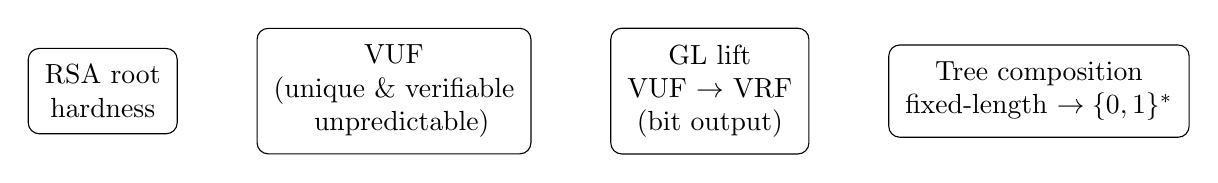
\begin{tikzpicture}[
  box/.style={draw, rounded corners, align=center, inner sep=6pt},
  arr/.style={-Latex, thick},
  node distance=10mm
]
\node[box] (rsa) {RSA root\\hardness};
\node[box, right=of rsa] (vuf) {VUF\\(unique \& verifiable\\\;\;unpredictable)};
\node[box, right=of vuf] (gl) {GL lift\\VUF $\to$ VRF\\(bit output)};
\node[box, right=of gl] (tree) {Tree composition\\fixed-length $\to \bits^\ast$};

\draw[arr] (rsa)   (vuf);
\draw[arr] (vuf)   (gl);
\draw[arr] (gl)   (tree);
\end{tikzpicture}
\end{center}

The remainder of this document:
\begin{itemize}
  \item defines the primitives and security games precisely enough to reason about them,
  \item gives the concrete RSA-based VUF (including the proof/verification mechanism),
  \item explains the GL lift and why it yields pseudorandomness from unpredictability (with the key reduction idea),
  \item gives the domain-extension construction and its security intuition,
  \item summarizes the overall theorem and typical costs (proof size, verification work).
\end{itemize}


\section{Notation and background primitives}


\paragraph{Efficient algorithms and negligible functions.}
All algorithms are probabilistic polynomial-time ($\ppt$) in the security parameter $k$.
A function $\negl:\N\to R_{\ge 0}$ is negligible if $\forall$ polynomials $p$ there exists $k_0$ such that for $k\ge k_0$,
$\negl(k) < 1/p(k)$.

\paragraph{Groups modulo an RSA modulus.}
Let $m=pq$ be an RSA modulus with distinct odd primes $p,q$.
Let $\Z_m$ denote integers modulo $m$ and $\Zstar{m}$ its multiplicative group of units.
Euler’s totient is $\varphi(m)=(p-1)(q-1)$.

\begin{lemma}[Permutation by exponentiation]
If $\gcd(e,\varphi(m))=1$, the map $\phi_e:\Zstar{m}\to\Zstar{m}$ defined by $\phi_e(z)=z^e \bmod m$ is a permutation.
\end{lemma}

\begin{proof}
Because $\gcd(e,\varphi(m))=1$, there exists $d$ with $ed\equiv 1\pmod{\varphi(m)}$.
Then for all $z\in\Zstar{m}$, $(z^e)^d=z^{ed}\equiv z\pmod m$ by Euler’s theorem,
so $\phi_d$ is the inverse of $\phi_e$.
\end{proof}

\paragraph{Inner product over $\mathbb{F}_2$.}
For $a,r\in\bits^b$,
\[
\ip{a}{r} \;=\; \sum_{i=1}^{b} a_i r_i \;\;(\mathrm{mod}\ 2).
\]


\section{Primitives: VRFs and VUFs}


\subsection{VRFs (syntax and properties)}
A VRF is a triple $(\Gen,\Eval,\Ver)$:

\begin{itemize}
  \item $\Gen(1^k)\to (\PK,\SK)$.
  \item $\Eval(\SK,x)\to (y,\pi)$ where $y$ is the function value and $\pi$ is a proof.
  \item $\Ver(\PK,x,y,\pi)\in\{0,1\}$ is the public verification algorithm.
\end{itemize}

\begin{definition}[Correctness and complete provability]
For all $x$ in the input domain, if $(\PK,\SK)\leftarrow\Gen(1^k)$ and $(y,\pi)\leftarrow\Eval(\SK,x)$, then
\[
\Pr[\Ver(\PK,x,y,\pi)=1] \ge 1-\negl(k).
\]
\end{definition}

\begin{definition}[Unique provability]
For any public key $\PK$ (even adversarially chosen) and any input $x$, there do not exist two distinct values $y\neq y'$
with proofs $\pi,\pi'$ such that $\Ver(\PK,x,y,\pi)=\Ver(\PK,x,y',\pi')=1$, except with negligible probability.
\end{definition}

\subsection{Residual pseudorandomness (the VRF security game)}
Informally: even after seeing many $\big(y,\pi\big)$ pairs at chosen inputs, the value at a fresh input looks random.

\begin{definition}[Residual pseudorandomness game]
Let $\mathcal{O}_{\SK}(x)$ return $(y,\pi)\leftarrow \Eval(\SK,x)$.
Adversary $\mathcal{A}$ gets $\PK$ and oracle access to $\mathcal{O}_{\SK}$, outputs a fresh $x^\star$ (never queried),
then receives either the real $y^\star$ or a uniform string of the same length; it may continue querying on inputs
$\neq x^\star$ and must guess which case it is in.
The advantage is
\[
\mathsf{Adv}^{\mathsf{vrf}}_{\mathcal{A}}(k)
= \left|\Pr[\mathcal{A}\ \text{guesses correctly}]-\tfrac12\right|.
\]
A VRF is secure if this advantage is negligible for all $\ppt{}$ adversaries.
\end{definition}

\subsection{VUFs: verifiable unpredictability}
The paper introduces a weaker primitive: a \emph{verifiable unpredictable function} (VUF).
The syntax, correctness, and unique provability are the same; the security goal is \emph{unpredictability} rather than
pseudorandomness.

\begin{definition}[Residual unpredictability (VUF security)]
Given $\PK$ and oracle access to $\mathcal{O}_{\SK}(x)=(y,\pi)$, no $\ppt{}$ adversary can output a fresh input $x^\star$
and a pair $(y^\star,\pi^\star)$ such that $\Ver(\PK,x^\star,y^\star,\pi^\star)=1$, except with negligible probability.
\end{definition}

\begin{remark}
A VUF is closely aligned with a \emph{unique} signature scheme where the signature is the proof and the message is the input.
The uniqueness condition matches unique provability.
\end{remark}


\section{Hardness assumption used by the construction}


\subsection{RSA root-extraction with random large prime exponent}
The core assumption is that extracting $p$-th roots modulo an RSA modulus is hard when $p$ is a random large prime.

\begin{definition}[RSA root hardness (informal)]
Let $m$ be an RSA modulus of size $\approx k$ bits, let $x\leftarrow \Zstar{m}$ be uniform, and let $p$ be a random
$(k+1)$-bit prime (hence $p>m$).
Given $(m,x,p)$, it is hard for any $s(k)$-time adversary to find $y$ such that
\[
y^p \equiv x \pmod m.
\]
\end{definition}

\paragraph{Why $p>m$ is useful for VRFs.}
Because $p>m>\varphi(m)$ and $p$ is prime, we have $\gcd(p,\varphi(m))=1$, so the $p$-th root in $\Zstar{m}$ (if it exists)
is \emph{unique}. This uniqueness is exactly what the construction exploits to satisfy unique provability.


\section{Construction 1: RSA-based VUF (value and proof)}


\subsection{High-level idea}
Fix a public element $r\in\Zstar{m}$. For each input $x$, associate a (publicly computable) prime exponent $p_x$.
Define the function value to be the unique $p_x$-th root of $r$:
\[
v_x := r^{1/p_x} \pmod m.
\]
The proof is simply the witness $v_x$ itself, and verification checks $v_x^{p_x}\equiv r \pmod m$.

\subsection{Prime indexing: $x \mapsto p_x$}
The construction needs a public map sending each $x$ to a (nearly always distinct) prime $p_x$ of about $(k+1)$ bits.
The paper uses a \emph{prime-sequence generator} (based on limited-independence polynomials and primality testing coins)
to ensure that with overwhelming probability, all $p_x$ are prime and distinct over the intended domain.

For this summary, treat the following as a black box:

\begin{quote}
\textbf{Prime Indexer $\mathsf{Prime}(x)$:} a public deterministic algorithm (given some public seed)
that outputs a $(k+1)$-bit prime $p_x$ for each input $x$, and outputs distinct primes for distinct $x$
except with negligible probability.
\end{quote}

\subsection{Algorithms}
\paragraph{Key generation.}
\[
\Gen(1^k):
\quad
\text{pick RSA modulus } m=pq;\ \text{pick } r\leftarrow\Zstar{m};\ \text{publish seed for }\mathsf{Prime}(\cdot).
\]
Public key:
\[
\PK=(m,r,\mathrm{seed}),\qquad \SK=(\PK,\varphi(m)).
\]

\paragraph{Evaluation (value + proof).}
On input $x$:
\[
p_x := \mathsf{Prime}(x),\qquad
d_x := p_x^{-1}\bmod \varphi(m),\qquad
v := r^{d_x}\bmod m,\qquad \pi := v.
\]
Output $(v,\pi)$ (the proof is the same element).

\paragraph{Verification.}
On $(x,v,\pi)$ (with $\pi=v$):
\begin{enumerate}
  \item Compute $p_x:=\mathsf{Prime}(x)$; verify $p_x$ is prime (with fresh randomness) and enforce $p_x>m$.
  \item Check $v\in\Zstar{m}$ and
  \[
  v^{p_x} \equiv r \pmod m.
  \]
  \item Accept iff all checks pass.
\end{enumerate}

\subsection{A compact correctness/uniqueness picture}

\begin{figure}[h]
\centering
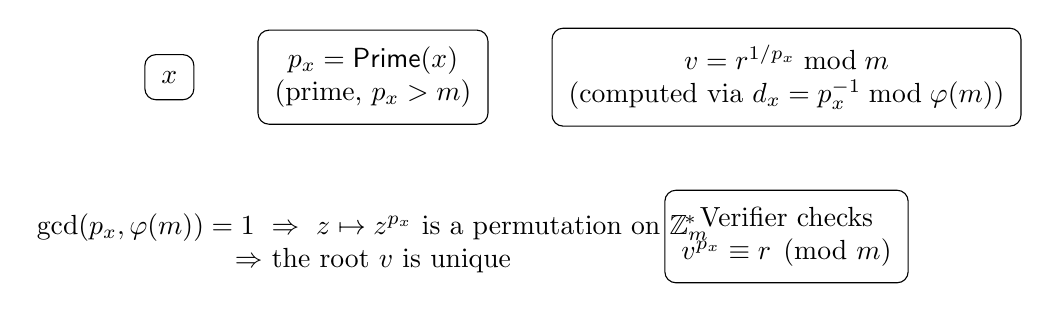
\begin{tikzpicture}[
  node distance=8mm,
  box/.style={draw, rounded corners, align=center, inner sep=6pt},
  arr/.style={-Latex, thick}
]
\node[box] (inp) {$x$};
\node[box, right=of inp] (px) {$p_x=\mathsf{Prime}(x)$\\(prime, $p_x>m$)};
\node[box, right=of px] (val) {$v=r^{1/p_x}\bmod m$\\(computed via $d_x=p_x^{-1}\bmod\varphi(m)$)};
\node[box, below=of val] (chk) {Verifier checks\\$v^{p_x}\equiv r\pmod m$};

\draw[arr] (inp)   (px);
\draw[arr] (px)   (val);
\draw[arr] (val)   (chk);

\node[align=center, below=10mm of px] (uniq) {$\gcd(p_x,\varphi(m))=1 \ \Rightarrow\ z\mapsto z^{p_x} \text{ is a permutation on }\Zstar{m}$\\
$\Rightarrow$ the root $v$ is unique};
\end{tikzpicture}
\caption{RSA-based VUF: the ``proof'' is the root $v$ itself; verification is one modular exponentiation.}
\end{figure}

\subsection{Core properties and their proofs}

\begin{lemma}[Completeness]
If $(v,\pi)\leftarrow \Eval(\SK,x)$ then $\Ver(\PK,x,v,\pi)=1$ except with negligible probability.
\end{lemma}

\begin{proof}
Let $p=p_x$ and $d=d_x$ with $pd\equiv 1\pmod{\varphi(m)}$, so $pd=1+t\varphi(m)$ for some integer $t$.
Then $v=r^d$ satisfies
\[
v^{p}\equiv (r^d)^p = r^{pd} = r^{1+t\varphi(m)} \equiv r\cdot (r^{\varphi(m)})^t \equiv r \pmod m,
\]
since $r\in\Zstar{m}$ implies $r^{\varphi(m)}\equiv 1\pmod m$.
\end{proof}

\begin{lemma}[Unique provability]
For any $\PK$ and input $x$, there is at most one $v\in\Zstar{m}$ such that $v^{p_x}\equiv r\pmod m$
(except with negligible probability due to primality-test error).
\end{lemma}

\begin{proof}
Verification enforces that $p_x$ is prime and $p_x>m$, hence $p_x\nmid \varphi(m)$ because $\varphi(m)<m$.
Thus $\gcd(p_x,\varphi(m))=1$ and exponentiation by $p_x$ is a permutation on $\Zstar{m}$.
A permutation has at most one preimage for $r$, so at most one $v$ can satisfy $v^{p_x}\equiv r$.
\end{proof}

\subsection{Residual unpredictability: the reduction structure}
The key security statement: producing a correct $(v,\pi)$ for a fresh $x^\star$ is as hard as extracting a root with a
fresh exponent. The paper’s reduction uses two central ingredients:

\begin{enumerate}
  \item \textbf{Programming one exponent:} choose a target $x^\star$ and construct the public seed so that
  $p_{x^\star}=p$ where $p$ is the RSA challenge exponent (while keeping the seed distribution close to honest).
  \item \textbf{Algebraic simulation:} set $r:=u^{E}\bmod m$ where $u$ comes from the RSA challenge and
  $E=\prod_{x\neq x^\star} p_x$. Then for any $x\neq x^\star$ one can answer the oracle query by outputting
  \[
  v_x := u^{E/p_x}\bmod m,
  \]
  since $(v_x)^{p_x}=u^{E}=r$.
\end{enumerate}

If the adversary outputs a valid $v^\star$ for $x^\star$, then $ (v^\star)^p = r = u^E$.
Using Bézout coefficients $\alpha,\beta$ with $\alpha E + \beta p =1$, one extracts $u^{1/p}$ as
\[
u^{1/p} \equiv (v^\star)^{\beta}\cdot u^{\alpha}\pmod m.
\]

\begin{theorem}[RSA-based VUF security (informal)]
Assuming RSA root-extraction is hard for random large primes, the above construction is a secure VUF:
any $\ppt{}$ adversary that forges a valid value at a fresh input with non-negligible probability yields an RSA-root inverter
with non-negligible probability (up to the standard ``guess the challenge input'' factor when selecting $x^\star$).
\end{theorem}


\section{Construction 2: Lifting VUFs to VRFs via Goldreich Levin}


\subsection{Construction (bit-valued VRF)}
Let the VUF output be encoded as a $b$-bit string $v(x)\in\bits^b$.
Sample a public random $r\in\bits^b$ and define the derived output bit:
\[
y(x) := \ip{v(x)}{r}\bmod 2.
\]

Evaluation returns a proof that reveals $v(x)$ and proves it is correct:
\[
\Eval'(\SK,x):\ (v,\pi)\leftarrow\Eval(\SK,x),\quad y=\ip{v}{r},\quad \pi'=(v,\pi).
\]
Verification checks both:
\[
\Ver'(\PK',x,y,\pi')=1 \iff \Big(\Ver(\PK,x,v,\pi)=1\Big)\ \wedge\ \Big(y=\ip{v}{r}\Big),
\]
where $\PK'=(\PK,r)$ and $\pi'=(v,\pi)$.

\subsection{Why this yields pseudorandomness (proof idea)}
Goldreich Levin (GL) says: if you can predict $\ip{w}{r}$ for random $r$ with noticeable advantage, you can reconstruct $w$
with non-negligible probability (using $\poly(k)$ queries to the predictor).

Here, the role of $w$ is played by $v(x^\star)$ at a fresh input $x^\star$.
So, if an adversary distinguishes $y(x^\star)$ from uniform, one can convert it into a predictor for $\ip{v(x^\star)}{r}$,
then apply GL reconstruction to recover $v(x^\star)$ itself. But recovering $v(x^\star)$ (together with its proof)
breaks the VUF unpredictability.

The technical nuisance addressed in the paper: the adversary chooses $x^\star$ adaptively, while GL wants a \emph{fixed}
$w=v(x^\star)$. The reduction handles this by choosing a random $x^\star$ and hoping it matches the adversary’s exam point
(the familiar $2^{-|x|}$ loss), motivating an initial ``short-input'' regime; the next construction removes this restriction.

\begin{figure}[h]
\centering
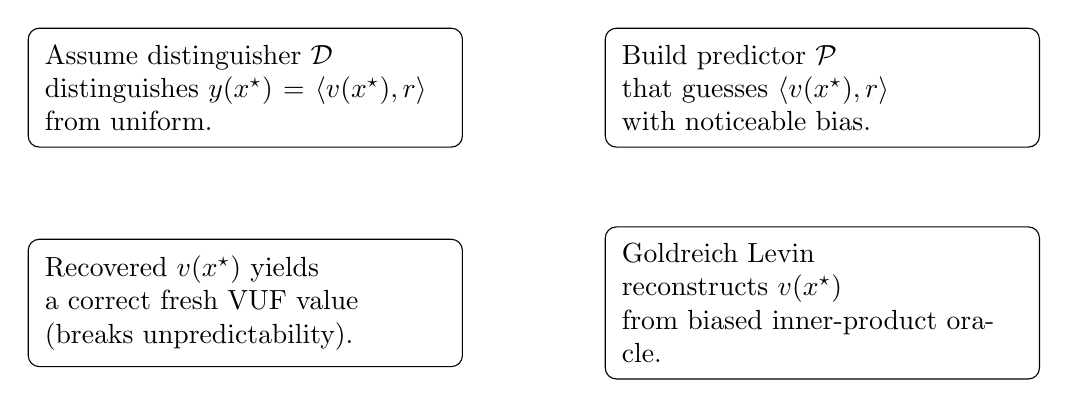
\begin{tikzpicture}[
  box/.style={draw, rounded corners, align=left, inner sep=6pt, text width=0.42\linewidth},
  arr/.style={-Latex, thick},
  node distance=10mm
]
\node[box] (dist) {Assume distinguisher $\mathcal{D}$\\distinguishes $y(x^\star)=\ip{v(x^\star)}{r}$ from uniform.};
\node[box, right=18mm of dist] (pred) {Build predictor $\mathcal{P}$\\that guesses $\ip{v(x^\star)}{r}$\\with noticeable bias.};
\node[box, below=of pred] (gl) {Goldreich Levin\\reconstructs $v(x^\star)$\\from biased inner-product oracle.};
\node[box, left=18mm of gl] (vuf) {Recovered $v(x^\star)$ yields\\a correct fresh VUF value\\(breaks unpredictability).};

\draw[arr] (dist)   (pred);
\draw[arr] (pred)   (gl);
\draw[arr] (gl)   (vuf);
\end{tikzpicture}
\caption{Security flow for the GL lift: distinguisher $\Rightarrow$ predictor $\Rightarrow$ GL reconstruction $\Rightarrow$ VUF break.}
\end{figure}

\begin{theorem}[VUF $\Rightarrow$ VRF (informal)]
If $(\Gen,\Eval,\Ver)$ is a secure VUF with unique provability, then the GL-derived $(\Gen',\Eval',\Ver')$ is a
(bit-valued) VRF for an appropriate parameter regime (with polynomial overhead and the standard challenge-point guessing loss).
\end{theorem}


\section{Construction 3: Extending the input domain to \texorpdfstring{$\bits^\ast$}{\{0,1\}*}}


\subsection{Tree-based composition}
Assume a base VRF (or verifiable pseudorandom predicate) that can be applied iteratively.
The idea is to label a binary tree so that each node label deterministically defines its children via the base VRF.

Conceptually:
\begin{itemize}
  \item Root has label $L(\epsilon)$.
  \item For a node with label $L(w)$, define
  \[
  L(w0) := f(L(w),0),\qquad L(w1) := f(L(w),1),
  \]
  where $f$ is a base VRF/predicate-to-string variant.
  \item For $x=b_1\cdots b_t$, the output is $L(x)$, the label at the end of the path.
\end{itemize}

\subsection{Proof structure}
A proof for $x=b_1\cdots b_t$ contains the intermediate labels and per-edge proofs:
\[
\big(L(b_1),\pi_1\big),\ \big(L(b_1b_2),\pi_2\big),\ \dots,\ \big(L(b_1\cdots b_t),\pi_t\big),
\]
where $\pi_i$ proves that $L(b_1\cdots b_i)$ was computed correctly from $L(b_1\cdots b_{i-1})$ and bit $b_i$.

\subsection{Prefix-free encoding}
To prevent revealing values on prefixes of future challenges, the input $x$ is first mapped to a prefix-free encoding
$\widehat{x}$ (so no $\widehat{x}$ is a prefix of $\widehat{x}'$ for $x\neq x'$).
The tree walk is done on $\widehat{x}$ instead of $x$.

\begin{figure}[h]
\centering
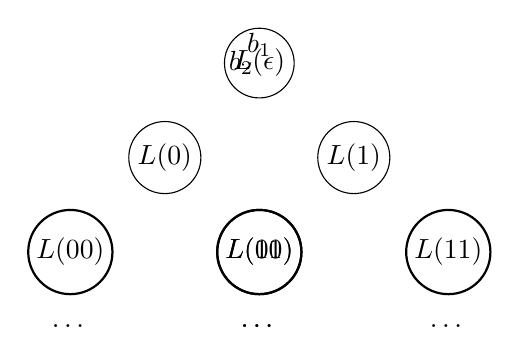
\begin{tikzpicture}[
  level distance=12mm,
  sibling distance=24mm,
  every node/.style={draw, circle, inner sep=1.5pt},
  edge from parent/.style={-Latex, thick},
  lab/.style={draw=none, rectangle, inner sep=2pt}
]
\node (root) {$L(\epsilon)$}
  child {node (l) {$L(0)$}
    child {node (ll) {$L(00)$}}
    child {node (lr) {$L(01)$}}
  }
  child {node (r) {$L(1)$}
    child {node (rl) {$L(10)$}}
    child {node (rr) {$L(11)$}}
  };

\node[lab, below=3mm of ll] {$\dots$};
\node[lab, below=3mm of lr] {$\dots$};
\node[lab, below=3mm of rl] {$\dots$};
\node[lab, below=3mm of rr] {$\dots$};

\path (root)   (r) node[midway, lab, above] {$b_1$};
\path (r)   (rl) node[midway, lab, left] {$b_2$};
\end{tikzpicture}
\caption{Domain extension: compute $L(\widehat{x})$ by walking the tree. Proofs certify each edge transition.}
\end{figure}

\subsection{Security idea (what must be shown)}
Fix an adversary that sees many path proofs and then challenges on a fresh $\widehat{x}$.
Two complementary arguments are used:

\begin{itemize}
  \item \textbf{Conditioned-on-no-collisions:} if no label repeats among nodes revealed so far, then the challenge label is
  distributed like a fresh base-VRF output at an unseen point, hence pseudorandom.
  \item \textbf{Collisions are unlikely (or exploitable):} if label repetitions happen with noticeable probability, one can
  leverage the first collision to predict a new label and contradict the base VRF security (label lengths are chosen to push
  collision probability down, and any non-negligible collision probability yields a distinguisher/predictor).
\end{itemize}

\begin{theorem}[Fixed-length $\Rightarrow$ unrestricted-length VRF (informal)]
Given a secure fixed-length VRF with sufficiently long labels (output length), the tree construction (with prefix-free encoding)
yields a secure VRF on $\bits^\ast$, with proof size and verification time linear in $|\widehat{x}|$.
\end{theorem}


\section{Summary tables (what each step guarantees)}


\subsection{Primitive checklist}
\begin{table}[h]
\centering
\renewcommand{\arraystretch}{1.15}
\begin{tabular}{@{}lccc@{}}
\toprule
\textbf{Primitive} & \textbf{Verifiable?} & \textbf{Unique proof?} & \textbf{Security goal} \\
\midrule
VUF & yes & yes & unpredictability at fresh points \\
VRF & yes & yes & pseudorandomness at fresh points \\
Tree-extended VRF & yes & yes & pseudorandomness on $\bits^\ast$ \\
\bottomrule
\end{tabular}
\caption{Conceptual distinction: VUF vs.\ VRF.}
\end{table}

\subsection{Construction and cost overview}
\begin{table}[h]
\centering
\renewcommand{\arraystretch}{1.2}
\begin{tabular}{@{}p{0.26\linewidth}p{0.34\linewidth}p{0.34\linewidth}@{}}
\toprule
\textbf{Step} & \textbf{What is built} & \textbf{Main cost} \\
\midrule
RSA $\Rightarrow$ VUF &
$v_x=r^{1/p_x}\bmod m$ with proof $\pi=v_x$ &
One exponentiation for verify; indexer computes $p_x$ \\
GL lift &
Bit output $y=\ip{v}{r}$ with proof revealing $v$ &
Proof includes $v$ (and VUF proof), plus GL reduction overhead \\
Tree extension &
VRF on $\bits^\ast$ via path labels and proofs &
Proof size $\Theta(|\widehat{x}|)$; verify $\Theta(|\widehat{x}|)$ \\
\bottomrule
\end{tabular}
\caption{Each reduction adds structure (and typically proof length) while preserving verifiability and uniqueness.}
\end{table}


\section{End-to-end statement (what you obtain)}


\begin{theorem}[End-to-end outcome (informal)]
Assuming RSA root-extraction is hard for random large prime exponents, there exists a VRF family on inputs $\bits^\ast$
that outputs at least one pseudorandom bit together with a publicly verifiable, uniquely valid proof of correctness.
The construction is explicit: RSA-based VUF $\Rightarrow$ GL-derived verifiable pseudorandom predicate $\Rightarrow$
tree-based domain extension.
\end{theorem}

\section{Practical reading notes (what to remember)}
\begin{itemize}
  \item \textbf{The proof is not a separate object in the RSA VUF:} the witness $v_x$ \emph{is} the proof.
  \item \textbf{Uniqueness is structural, not heuristic:} enforcing $p_x$ prime and $p_x>m$ makes exponentiation a permutation.
  \item \textbf{Security reductions have two recurring motifs:}
    (i) \emph{program a special input} and pay a ``guess the challenge'' loss,
    (ii) \emph{algebraic simulation} that answers all other queries consistently without knowing secret structure.
  \item \textbf{Domain extension trades interaction for proof length:} proofs grow linearly with input length.
\end{itemize}

\end{document}
